\section{Results}\label{res}

The following results were obtained using the ChiVO (Chilean Virtual Observatory) datacenter \citep{solar2015chilean} on an Intel Xeon CPU E5-2680 2.50GHz with 12 cores and 64 GB of RAM.
For all the experiments we set $T=300$ and set the dimension of the encoder representation $D$ to $16$,  generating a 95\% of compression.

\subsection{Quality Evaluation} 

%reconstruction + denoising table  + residual..
\begin{table}[!t]
\caption{Reconstruction and denoising results with associated metrics by different methods. The configuration of the passband corresponds to low and high pass filters respectively, while for moving average corresponds to window size. The Mandel Agol simulation has the library on Config column, while deep AE methods have the dimension of the encoder/latent representation.}
\label{tab:rec_results}
\centering
\begin{tabular}{|c|c|cc|cc|c|} \cline{3-7}
\multicolumn{1}{c}{} &         & \multicolumn{2}{c|}{\textit{Reconstruction}} & \multicolumn{2}{c|}{\textit{Denoising}} & \textit{Residual Noise} \\ \hline
\multicolumn{1}{|c|}{\textbf{Method}}  & \textbf{Config.}   & \textbf{RMSE}         & \textbf{MAE}         & \textbf{AutoC}   & \textbf{Diff-M}   & \textbf{Spectral-H}            \\ \hline \hline
\multicolumn{2}{|c|}{Original LC}   & -  &  -   & 0.27                & 0.78              &  0.84    \\ \hline \hline
\multicolumn{1}{|c|}{\multirow{3}{*}{Passband}}  & 1-500  & 1.08  & 0.62   & 0.97  & 0.05  &  0.82 \\ %\cline{2-7}
     & 50-1500 & 1.04    & 0.65 & 0.83  & 0.20  &   0.84       \\ %\cline{2-7} 
    & 50-2500 & 0.96     & 0.64     & 0.67  & 0.36     &    0.85     \\ \hline
\multicolumn{1}{|c|}{\multirow{3}{*}{Mov. avg}} & 3 & 0.72   & 0.46 & 0.70 & 0.27 &  0.88     \\ %\cline{2-7} 
      & 5       & 0.84   & 0.51  & 0.78  & 0.17    &   0.86            \\ %\cline{2-7} 
   & 10      & 0.94       & 0.55  & 0.84    & 0.09   &  0.84  \\ \hline
M-A sim & \textit{batman}    & 2.34     & 0.63         & 0.64        & 0.22         & 0.89          \\ \hline
RAE$_t$ & 16        & 0.69       & 0.48   & 0.50    & 0.13     &     0.90        \\ \hline
\textbf{VRAE$_t$} & 16  & 0.69     & 0.48  & 0.59  & 0.07     &    0.90               \\ %\hline
\textbf{S-VRAE$_t$}  & 16    & 0.72   & 0.49  & 0.61   & 0.06     &     0.90     \\ \hline
\end{tabular}
\end{table}
The reconstruction and smoothing scores for different methods and configurations are presented on Table \ref{tab:rec_results}.
As expected, passband methods offer a very good denoising behavior, but fails to reconstruct properly the signal. For example, if we vary the filter on passband, specifically narrows the pass frequency, the reconstruction error increases and it gets smother (high Autocorr and low Diff-M). 
The same effect occurs for moving average method when we increase the window size. Compared to passband, the moving average method presents lower reconstruction errors but producing a rougher time series (low AutoC).
The Mandel-Agol simulation has a very high reconstruction error compared to other methods, this is because it performs a perfect simulation without any noise of the light curve original measures. The simulation function does not consider any smoothness, as it models the ideal behavior of the transit objects. Nevertheless, the auto-correlation is still strong as in the previous methods.

It is clear that learning-based methods (autoencoders) have the lowest reconstruction errors, only comparable with moving average with window size of 3. Also, the reconstructed data is still significantly smoother than the original time series (\textit{denoising effect}). Between them, variational proposals have a higher auto-correlation (smoother) than its deterministic counterpart RAE$_t$. They even have the lowest difference on consecutive values (Diff-M) of all methods, showing smoother transitions on the local behavior of the time series. 

Adding the re-scaling into the model (S-VRAE$_t$) seems to produce a smoother reconstructed time series but with the cost of increasing the reconstruction error, but both results are quite similar. The disadvantage in reconstruction is expected because the model needs to learn simultaneously to codify and reconstruct the scale of the data.

If we take a look to the spectral entropy of the residual, we clearly identify that learning-based methods exhibit the best scores. This mean that these methods really focus on learning the time series patterns to perform the reconstruction, instead of removing structure for achieving high smoothness like in the generic denoising methods presented.  %denosiing temporal
Please note that the spectral entropy has a reference value of $0.84$ (i.e., on the original light curve) and its maximum value is $1.0$ (i.e., a uniform distribution of frequencies). Therefore, the learning-based methods (followed closely by the Mandel-Agol simulation) are actually removing unstructured patterns from the light-curves.

\begin{figure}[!t]
    \centering
    \begin{tabular}{c}
         (a) Mandel-Agol simulation \\ 
         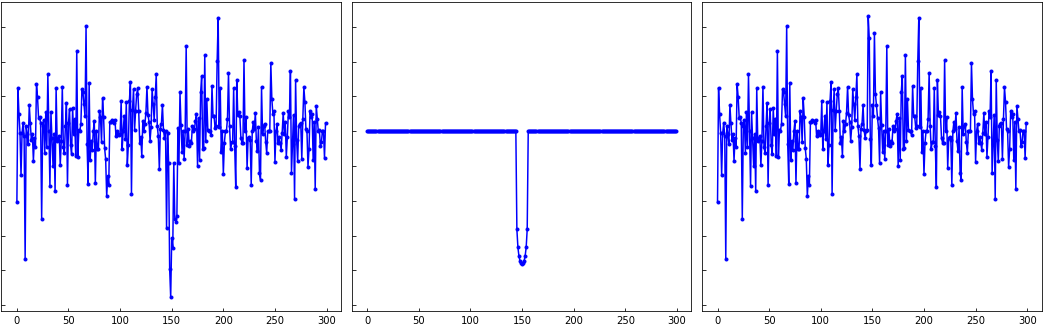
\includegraphics[width=0.95\textwidth, height=2cm]{imgs/MA_1.png} \\
         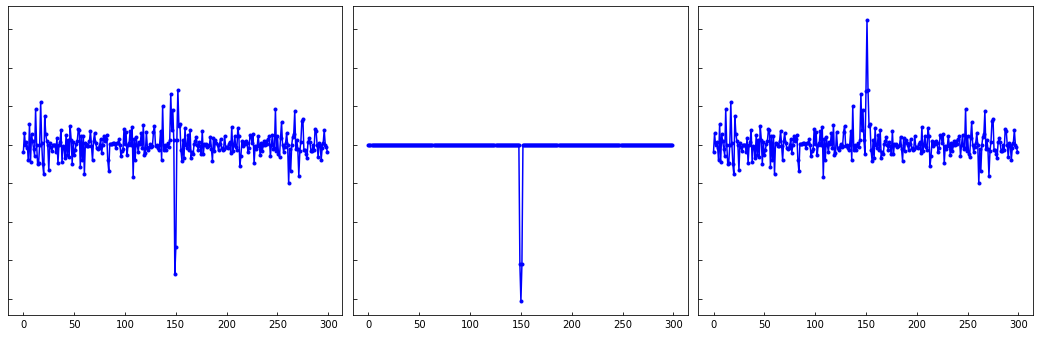
\includegraphics[width=0.95\textwidth, height=2cm]{imgs/MA_2.png} \\
        (b) RAE$_t$ \\
         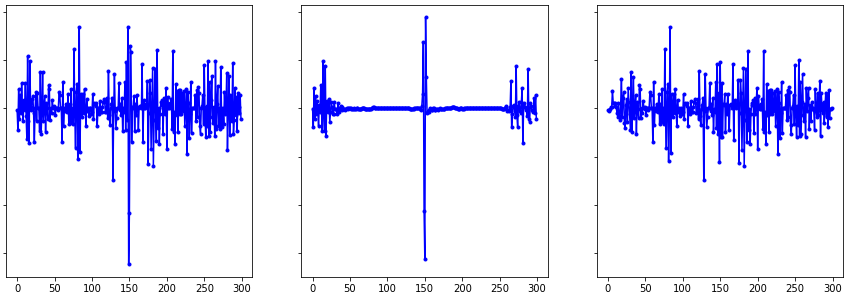
\includegraphics[width=0.95\textwidth, height=2cm]{imgs/RAE_1.png}  \\
         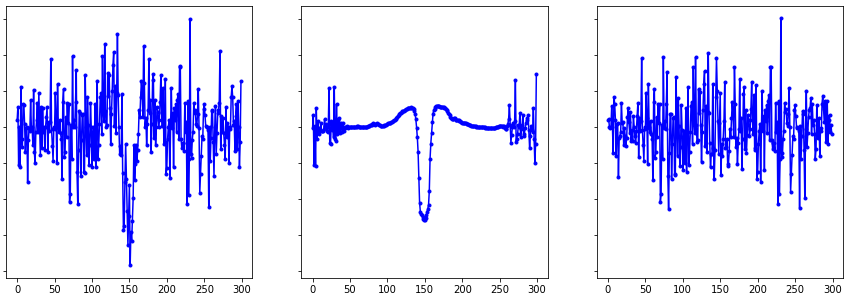
\includegraphics[width=0.95\textwidth, height=2cm]{imgs/RAE_2.png}  \\
        (c) \textbf{S-VRAE$_t$} \\ 
         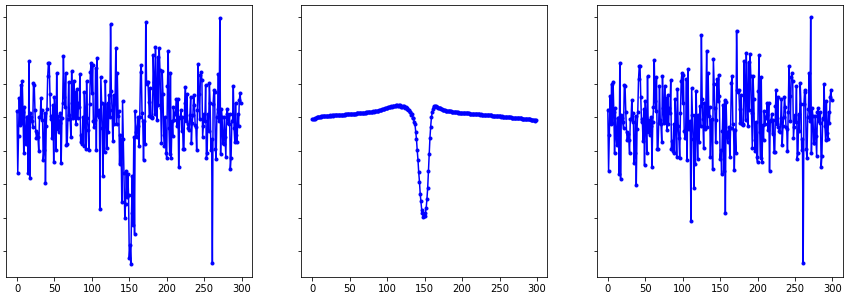
\includegraphics[width=0.95\textwidth, height=2cm]{imgs/S-VRAE_1.png} \\
         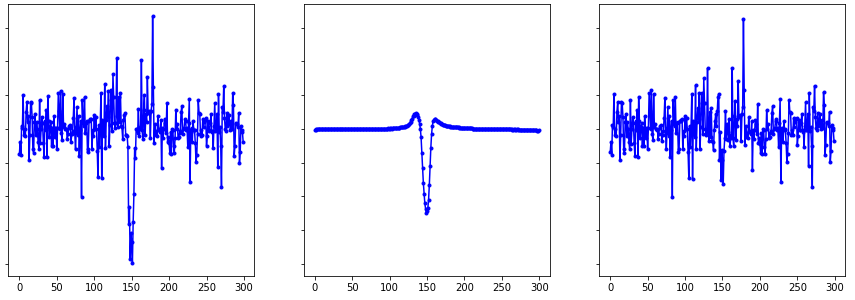
\includegraphics[width=0.95\textwidth, height=2cm]{imgs/S-VRAE_2.png} \\
    \end{tabular}
    \caption{Examples of a random reconstructed light curve. The method in (a) correspond to the M-A simulation \citep{mandel2002analytic}, in (b) is the deterministic counterpart of our proposal \citep{naul2018recurrent} and in (c) one of the proposals. The first column is the original folded-global raw light curve, the second is the reconstructed or denoised, and finally the third column correspond to the residual}
    \label{fig:denois_ex}
\end{figure}
%We visualize the denoising process of the reconstructed or generated time series, including the residual, on
Figure \ref{fig:denois_ex} shows a few examples of reconstructed light curves for understanding better the previous results. The RAE$_t$ approach tend to keep the noise on the edges of the time series (in order to perform a good reconstruction), while our proposal (S-VRAE$_t$) generates denoised transits to the extent of being comparable with Mandel Agol simulation. The VRAE$_t$ model is not shown because visually it is quite similar to S-VRAE$_t$.
On the other hand, the Mandel Agol simulation residuals show that the errors are related to the positives values, as the function models that the measured light could not be greater than the regular/normal light intensity (without eclipsing objects) of the star, i.e. is limited by the model itself.

\begin{table}[!t]
\caption{Pearson correlation (Pcorr) between features, this express the linear dependence of all features on the representations, while Pcorr-A is the absolute mean. Mutual Information (MI) between the features, this express an approximation to the information dependence of all features on the representation, while N-MI is a normalized value between 0 and 1. All the representations are generated with 16 dimensions, except metadata that has 10 features.}
\label{tab:feat_dep}
\centering
\begin{tabular}{c|cc|cc} \hline
\textbf{Representation} & \textbf{Pcorr} & \textbf{Pcorr-A} & \textbf{MI} & \textbf{N-MI} \\ \hline
Metadata     & $0.064$ & $0.162$ & $0.275$ & $0.044$ \\ \hline
(Raw) F+PCA  & $0.000$ & $0.000$ & $0.210$ & $0.027$ \\ %\hline
(Fold) F+PCA & $0.000$ & $0.000$ & $0.061$ & $0.008$ \\ \hline
RAE$_t$  &  $0.057$ & $0.277$  & $0.255$ & $0.033$  \\ %\hline
\textbf{VRAE$_t$}   &  $0.012$ & $0.168$ & $0.122$ & $0.016$   \\ %\hline
\textbf{S-VRAE$_t$}   &  $-0.003$ & $0.138$ & $0.072$ & $0.009$  \\ \hline
\end{tabular}
\end{table}
%algo un pcoo extraño: correlación es mas alta que MI -> debe ser por la aproximación del cálculo
In Table \ref{tab:feat_dep} we present the feature dependence of the generated representations. 
Here it can be seen that learning-based methods (AEs) obtain features with less information duplicity than the metadata features obtained by Kepler. Minimizing the correlation and mutual information could simplify the task of identifying independent linear and non-linear processes in the system respectively. 

We compute a \textit{Fourier plus PCA} (F+PCA) representation from the raw measurements and from the folded representation. Both obtained components that are linearly independent between them based on the orthogonality of PCA formulation. However, the F+PCA method over fold representation produces less mutual information, being an example of optimal independence for the problem.
The closer values to F+PCA (fold) are from the proposed model with re-scaling (S-VRAE$_t$), showing the good impact of including the scale into the model. It is worth noting that the variational proposed models (VRAE$_t$ and S-VRAE$_t$) learn a space with more independent components (linearly and based on mutual information) than the deterministic counterpart RAE$_t$. 

%The dependence results (Table \ref{tab:feat_dep}) is an abstract visualization of the learned space or manifold. 
Table \ref{tab:feat_dep} illustrates that, through the variational features of the proposed models, more exclusive information could be stored (as every feature represent a more different structure) and used for different propose, as its shown in the following.

%\subsection{Encoder evaluation} 
\subsection{Application of the Learned Representation} 

%The learned embeddings (representation) can be used to perform a classification of the . 
\begin{table}[!t]
\caption{Classification performance on the representation generated by different methods and techniques. The F1 score desegregated by the classes of the problem is presented too.}
\label{tab:class_results}
\centering
\begin{tabular}{c|c|cc|c} \hline %\cline{3-4} 
\textbf{Representation} & \textit{input dim} & \textbf{Non-exoplanet} & \textbf{Exoplanet} & \textbf{F1-Ma} \\ \hline
Metadata   & $10$  & $90.13$ & $83.85$  & $87.00$   \\ %\hline %-- non-folded
Folded-Global & $T=300$ & $83.51$  & $69.36$  & $76.45$ \\ \hline
\multicolumn{5}{c}{\textit{Unsupervised Methods}} \\ \hline
(Raw) F+PCA    & $16$ & $77.14$  & $71.21$ & $68.66$ \\ %o sacar
(Fold) F+PCA  & $16$ & $84.62$  & $71.34$ & $77.98$ \\
RAE$_t$  & $16$  & $84.42$ & $72.40$  & $78.41$    \\ %\hline
\textbf{VRAE$_t$}   & $16$  & $85.88$ & $74.84$  & $80.36$   \\ %\hline
\textbf{S-VRAE$_t$} & $16$  & $87.39$ & $77.91$  & $82.65$     \\ \hline
\multicolumn{5}{c}{\textit{Supervised Methods}} \\ \hline %-- folded
RNN$_t$ & $T=300$  & $88.67$ & $79.09 $ & $83.87$   \\ %\hline
1D CNN  & $T=300$ & $89.27$  & $81.40$  & $85.33$  \\  %state of the art
\hline
\end{tabular}
\end{table}
A different way to assess the quality of a representation is to impose a task, in this case, classifying light-curves between transits exoplanets (confirmed) and other variability (false positive).
Table ~\ref{tab:class_results} presents the classification results by using a shallow feed forward network on the exoplanet binary detection problem. Here we compare different representations, including the learning-based methods (autoencoders) and supervised learning methods from the folded-global light curve representation (with $T$ bins). The ``1D CNN" is a supervised technique based on \citep{shallue2018identifying} work, while ``RNN$_t$" is basically the encoder model of RAE$_t$/VRAE$_t$ with a classification layer at the top, without decoder phase.

%comentarios generales
Table \ref{tab:class_results} shows that the unsupervised feature extraction methods are useful, based on the classification improvement over the the raw folded-global representation. This suggest that is easier to discriminate using these compressed representations than the raw measurements. Besides, the representation of 16 dimensions is computationally lighter, taking a fraction of the time to train the supervised FF network (i.e., $10\%$).
However, supervised methods that train an internal representation explicitly specialized for the task, have better classification results over all unsupervised techniques. Nevertheless, there is still some gaps of improvementment based on the performance of the experts domain defined features (metadata).
%diferencias entre metodos no supervisados
It can be seen that the representation of the variational extension (VRAE$_t$) gives an improvement on the classification with respect to the RAE$_t$ model. This can be explained due to the generalization capacity of the implemented latent variables within the variational model. 
Furthermore, the re-scale extension (S-VRAE$_t$) results suggest that the method extract more useful information from the light curve scale, being able to codify better patterns for the classification objective. Indeed, the S-VRAE$_t$ model has the best classification performance among unsupervised techniques, being very close to its maximum model capacity (the RNN$_t$ model performance).


%In summary, 3 key factors:
% - a better denoising effect
% - a better classification (more useful representation)
% - more independent features (more informative representation)

%K2

